\section{Lezioni del 09-10-11/05/2018}

\subsection{Programmazione Dinamica}

Da \href{https://it.wikipedia.org/wiki/Programmazione_dinamica}{Wikipedia}: 
\begin{quote}
    In Informatica la \emph{programmazione dinamica} è una tecnica di progettazione di algoritmi basata sulla divisione del problema in 
    sottoproblemi e sull'utilizzo di sottostrutture ottimali. 
\end{quote}

La programmazione dinamica è utilizzata in casi in cui i sottoproblemi vengono richiamati molte volte, rendendo
conveniente salvare in memoria il risultato di tali sottoproblemi per non doverli ricalcolare a ogni iterazione. Ad esempio, possiamo immaginare che i dati vengano
immagazzinati in una tabella:

\begin{center}
    \begin{tabular}{|c|c|c|}
        \hline
        $P_1$ & sol. $P_1$ & costo $P_1$ \\
        \hline 
        $P_2$ & sol. $P_2$ & costo $P_2$ \\
        \hline
        \dots & \dots & \dots \\
        \hline
    \end{tabular}    
\end{center}

\begin{enumerate}
    \item Caratterizzo la ``struttura'' della \emph{soluzione ottima} (soluzione ottima di $P$ in termini di soluzioni ottime di sottoproblemi);
    \item Espressione ricorsiva del \emph{valore} della soluzione ottima;
    \item Algoritmo che calcola il ``valore della soluzione ottima'':
    $$\Downarrow$$
    \[
        \begin{cases}
            \text{top down} \\
            \text{bottom up}
        \end{cases}
    \]
    \item Algoritmo che calcola la \emph{soluzione} e il \emph{valore}
\end{enumerate}

\subsubsection{Taglio delle aste}

Introduciamo la programmazione dinamica con un primo esempio. Ipotizziamo ci sia un'azienda che produce aste di metallo
molto lunghe, per venderle tagliate a pezzi.

Ogni pezzo ha un valore di vendita legato alla lunghezza. Voglio dei tagli che massimizzino il ricavo. Abbiamo
\begin{itemize}
    \item Lunghezza complessiva dell'asta $= n$;
    \item Prezzi $p_1, p_2, \dots , p_n$.
    \item $r_n$ Ricavo massimo ottenibile per l'asta di lunghezza $n$
\end{itemize}

\paragraph{Esempio} $n = 7$

\begin{center}
    \begin{tabular}{r|l|l|l|l|l|l|l}
        Lunghezza & 1 & 2 & 3 & 4 & 5 & 6 & 7 \\
        \hline
        $p_i$ & 1 & 5 & 8 & 9 & 10 & 17 & 17
    \end{tabular}
\end{center}
Come possiamo suddividere l'asta di lunghezza 7?

\begin{align*}
    \text{Suddivisione} & \rightarrow p_i \\
    1+1+ \dots +1 & \rightarrow 7 \\
    2+1+ \dots +1 & \rightarrow 10 \\
    2+2+2+1 & \rightarrow 16 \\
    7  & \rightarrow 17 \\
    6+1  & \rightarrow 18 \\
    2+2+3 & \rightarrow 18 \\
    \dots
\end{align*}
Sono possibili $2^{n-1}$ possibili combinazioni di tagli. È evidente che calcolarle tutte esplicitamente risulta estremamente inefficiente.

Supponiamo di tagliare l'asta in posizione $i$, tale che si ottenga una soluzione con due sottoproblemi ottimali (ottenendo le sotto-aste $a$ e $b$).

\begin{align*}
    r_n & = r_i + r_{n-i} \\
    r_n & = a + b \text{ con } a < r_i \\
    r_n' & = r_i + b > r_n \text{ (non ha particolare senso)} \\
    & i \text{ è ottimo?} \\
    r_0 & = 0 \\
    r_n & = max \left( \{ p_n \} \cup \{ r_i + r_{n-i} \ | \ i = 1 , \twodots, n-1 \} \right) \\
    & \qquad \text{($p_n$ non taglio, $r_{n-1}$ taglio, e ottimizzo le due parti)} \\
    & = max\{ p_i + r_{n-i} \ | \ i=1, \twodots, n \}
\end{align*}

\clearpage

\paragraph{Pseudocodice}
\begin{codebox}
    \Procname{$\proc{CutRod}(p,n)$}
\li \If $n = 0$
\li \Then \Return $0$
\li \Else
\li     $q \gets -1$
\li     \For $i = 1$ \To $n$
\li     \Do $q \gets \proc{Max}(q, P[i] + \proc{CutRod}(P,n-i))$ 
        \End
    \End
\li \Return $q$
\end{codebox}

\paragraph{Complessità}
\begin{align*}
    T(n) & = 1 + \displaystyle\sum_{i=1}^n T(n-i) \\
    & = 1 + \displaystyle\sum_{j=0}^{n-1} T(j) = \Theta(2^n) \\
    T(0) & = 1 + 0 = 1 = 2^0 \\
    T(n+1) & = 1 + \displaystyle\sum_{j=0}^n T(j) \\
    & = 1 + \displaystyle\sum_{j=0}^{n-1} T(n) + T(n) \qquad
    \left( \displaystyle\sum_{j=0}^{n-1} T(n) = T(n) \right) \\
    & = 2 T(n)
\end{align*}

\clearpage

Vediamo il problema della ripetizione dei sottoproblemi con $n = 4$
\begin{center}
    \begin{tikzpicture}
    \Tree
    [.$P4$
        [.${\color{red} P3}$
            [.${\color{green} P2}$ 
                [.${\color{blue} P1}$ 
                    [.${\color{cyan} P0}$ ]
                ]
                [.${\color{cyan} P0}$ ]
            ]
            [.${\color{blue} P1}$ 
                [.${\color{cyan} P0}$ ]
            ]
            [.${\color{cyan} P0}$ ]
        ]
        [.${\color{green} P2}$
            [.${\color{blue} P1}$ 
                [.${\color{cyan} P0}$ ]
            ]
            [.${\color{cyan} P0}$ ]
        ]
        [.${\color{blue} P1}$
            [.${\color{cyan} P0}$ ]
        ]
        [.${\color{cyan} P0}$ ]
    ]
    \end{tikzpicture}
\end{center}

Sfruttando la ``memoria'', restano i sottoproblemi risolti una sola volta:
\begin{center}
    \begin{tikzpicture}
    \Tree
    [.$P4$
        [.${\color{red} P3}$
            [.${\color{green} P2}$ 
                [.${\color{blue} P1}$ 
                    [.${\color{cyan} P0}$ ]
                    \edge[blank]; \node[blank]{};
                ]
                \edge[blank]; \node[blank]{};
            ]
            \edge[blank]; \node[blank]{};
        ]
        \edge[blank]; \node[blank]{};
    ]
    \end{tikzpicture}
\end{center}

\begin{itemize}
    \item \verb|#|sottoproblemi polinomiale ($n^k$) nella dimensione del problema di partenza;
    \item Esiste un algoritmo polinomiale per calcolare la soluzione del problema date le soluzioni dei sottoproblemi.
\end{itemize}

Sono possibili due approcci: 
\begin{itemize}
    \item Top-down con \emph{memoization};
    \item Bottom-up.
\end{itemize}

\paragraph{Top-down}
\begin{codebox}
    \Procname{$\proc{MemCutRod}(p,n)$}
\li \For $i \gets 1$ \To $n$
\li \Do $r[i] \gets -1$
    \End
\li \Return $\proc{MemCutRod}(p,n,r)$
\end{codebox}
\begin{codebox}
    \Procname{$\proc{MemCutRod-aux}(p,j,r)$}
\li \If $r[j] < 0$
\li \Then \If $j = 0$ 
\li     \Then $r[j] \gets 0$
\li     \Else 
\li         $q = -1$
\li         \For $i \gets 1$ \To $j$
\li         \Do $q \gets \proc{Max}(q, p[i]+\proc{MemCutRod-aux}(p,j-i,r))$
\li             $r[j] \gets q$
            \End
        \End
    \End
\li \Return $r[j]$
\end{codebox}

$$j = 1, \ldots, n$$
\begin{gather*}
    \displaystyle\sum_{j=1}^{n} \left( \Theta(1) + j \Theta(1) \right) \\
    = \Theta \left( \displaystyle\sum_{j=1}^{n} (1+j) \right) = \Theta(n^2)
\end{gather*}

\paragraph{Bottom-Up}
\begin{codebox}
    \Procname{$\proc{BottomUpCutRod}(p,n)$}
\li $\text{alloco } r[1 \twodots n]$
\li $r[0] \gets 0$
\li \For $j \gets 1$ \To $n$ \Comment calcolo $r[j]$
\li \Do $q \gets -1$
\li     \For $i \gets 1$ \To $j$
\li     \Do $q \gets \proc{Max}(q, p[i] + r[j-1])$ \Comment $\Theta(1)$
        \End
        $r[j] \gets q$
    \End
\li \Return $r[n]$
\end{codebox}

$$\displaystyle\sum_{i=1}^n \displaystyle\sum_{i=1}^j \Theta(1) = \Theta (n^2)$$

%10/05
\subsubsection{Prodotto di Matrici}

Ecco un altro esempio di \emph{programmazione dinamica}.

Consideriamo $A$ e $B$ di dimensioni $p \times q$ e $q \times r$
$\rightarrow$ otteniamo $C$ di dimensioni $p \times r$.

$$C[i,j] = \displaystyle\sum_{k=1}^q A[i,k] \cdot B[k,j]$$

$$costo = q \text{ prodotti di scalari per ogni elemento} = q\cdot p \cdot r$$

Vogliamo moltiplicare $n$ matrici $C = A_1 \times A_2 \times \ldots \times A_n$. 
Possiamo farlo in molti modi poich\'e è un'operazione associativa e vogliamo il modo che ci permetta di fare meno prodotti scalari possibili.

\paragraph{Esempio} 
$$A_1 \times A_2 \times A_3$$ 
$$A_1 \rightarrow 10 \times 100$$
$$A_2 \rightarrow 100 \times 5$$
$$A_3 \rightarrow 5 \times 50$$

Abbiamo due possibili \emph{parentetizzazioni}:
\begin{align*}
    (A_1 \times A_2) \times A_3 \qquad & (10 \times 100 \times 5) + 100 \times 5 \times 50 = 7500 \\
    A_1 \times (A_2 \times A_3) \qquad & 10 \times 100 \times 50 + (100 \times 5 \times 50) = 75000
\end{align*}
Non posso provare tutte le parentetizzazioni del prodotto perch\'e sono in numero

\[
    P(n) = 
    \begin{cases}
        1 & \text{se } n = 1 \\
        \displaystyle\sum_{k=1}^{n-1} P(k) P(n-k) & \text{se } n > 1
    \end{cases}
\]

Che cresce in maniera esponenziale! $\Omega(2^n)$
\begin{align*}
    P(n) & = \displaystyle\sum_{k=1}^{n-1} P(k) P(n-k) 
        \geq \displaystyle\sum_{k=1}^{n-1} c \cdot 2^k \cdot c \cdot 2^{n-k} \\
        & \geq (n-1)c^2 \cdot 2^n \geq c \cdot 2^n \text{ per } c \geq 1, \ n > 2
\end{align*}

\paragraph{Sottoproblema} $A_i \times \ldots \times A_j$, $1 \leq i < j \leq n$, in numero $\Theta(n^2)$
\begin{enumerate}
    \item Suppongo di avere la \textit{soluzione ottima}. Avrò un livello esterno di parentesizzazione
    $$(A_1 \times \ldots \times A_k)(A_{k+1} \times \ldots \times A_n)$$
    Ognuna delle due parentesizzazioni è ottima per quel sottoproblema.

    \textbf{Nota bene}: Ogni matrice $A_i$ ha dimensioni $p_{i-1} \times p_i$, quindi serve un array delle dimensioni $p[0\twodots n]$;

    \item Considero i sottoproblemi $A_{ij} = (A_1 \times A_2 \times \ldots \times A_j)$ \par
    Indico con $m[i,j]$ il valore della \emph{soluzione ottima} per il \textit{sottoproblema};
    \begin{align*}
        m[i,j] & = \text{minimo } \# \text{ di prodotti per calcolare } A_{ij} \\
        & =
        \begin{cases}
            0 & i = j \\
            min_{i \leq n < j} \left( m[i,k] + m[k+1,j] + p_{i-1} p_k p_j \right) & i < j
        \end{cases}
    \end{align*}
    È il minimo delle due parentesizzazioni + il costo del prodotto fra le due matrici ottenute.
\end{enumerate}

\paragraph{Pseudocodice}
\begin{codebox}
\Procname{$\proc{MatrixChain}(p,i,j)$}
\li \If $i = j$
\li \Then \Return $0$
\li \Else
\li     $\id{cmin} \gets +\infty$
\li     \For $k \gets i$ \To $j-1$
\li     \Do 
            $q \gets \proc{MatrixChain}(p,i,k) + \proc{MatrixChain}(p,k+1,j) + $
\zi         $\quad + p[i-1]p[k]p[j]$
\li         \If $q < \id{cmin}$
\li         \Then $\id{cmin} \gets q$
            \End
        \End
    \End
\li \Return $\id{cmin}$
\end{codebox}

\paragraph{Complessità} Mi aspetto poca efficienza.
\begin{align*}
    T(n) & = 1 + \displaystyle\sum_{k=1}^{n-1} \left( T(k) T(n-k) + 1 \right) \qquad && \left[ 1 \text{ costante qualsiasi} \right] \\
    & = n + 2\displaystyle\sum_{j=1}^{n-1}T(j) \quad && \left[ \text{trovo } T(k) \text{ due volte} \right] \\
    & = \Omega(2^n)
\end{align*}

\paragraph{Dimostrazione} per induzione (dimostrazione che $T(n) \geq 2 \ \forall n \geq 1$)

\begin{itemize}
    \item \textbf{Base}: $T(1) = 1 \geq 2^{1-1}$ ok;
    \item \textbf{Induzione}: 
    \begin{align*}
        T(n-1) & = n+1 +2 \displaystyle\sum_{j=1}^{n} T(j) = \\
        & = n+1+2\displaystyle\sum_{j=1}^{n-1} T(j) + 2T(n) \geq 
        2T(n) \geq 2^n
    \end{align*}
\end{itemize}

Anche in questo problema, i sottoproblemi vengono risolti molte volte. Ecco perch\'e è possibile un approccio alla programmazione
dinamica per migliorare notevolmente l'efficienza.

\begin{itemize}
    \item \textbf{Soluzione Top-down}: memorizzo in $m[i,j]$ la soluzione del sottopb $i,j$.
    \begin{codebox}
\Procname{$\proc{MatrixChain}(p,i,j)$}
\li \For $i \gets 1$ \To $n$
\li \Do 
        \For $j \gets 1$ \To $n$
\li     \Do
            $m[i,j] \gets +\infty$
        \End
    \End
\li \Return $\proc{MatrixChainRec}(p,1,n,m)$
\end{codebox}
    \begin{codebox}
\Procname{$\proc{MatrixChainRec}(p,i,j,m)$}
\li \If $m[i,j] = +\infty$
\li \Then \If $i = j$
\li     \Then
            $m[i,j] \gets 0$
\li     \Else 
\li         \For $k \gets 1$ \To $j-1$
\li         \Do
                $q \gets \proc{MatrixChainRec}(p,i,k,m)+$
\zi             $\quad + \proc{MatrixChainRec}(p,k+1,j,m)+$
\zi             $\quad + p[i-1]p[k]p[j]$
\li             \If $q < m[i,j]$
\li             \Then $m[i,j] \gets q$
                \End
            \End
        \End
    \End
\li \Return $m[i,j]$
\end{codebox}
    Per ogni coppia $(i,j)$ ho un ciclo di costo $O(n)$ e ho $n^2$ coppie
    $$\Rightarrow \text{complessità } O(n^3)$$

    %11/05
    \item \textbf{Soluzione Bottom-up} \par
    per lunghezza \underline{crescente} della sequenza $A_i \twodots A_j$
    \begin{codebox}
\Procname{$\proc{MatrixChain}(p,n)$}
\li \For $i \gets 1$ \To $n$
\li \Do 
        $m[i,j] \gets 0$
    \End
\li \For $l \gets 2$ \To $n$
\li \Do \For $i \gets 1$ \To $n-l+1$
\li     \Do
            $j \gets i+l-1$
\li         $m[i,j] \gets +\infty$
\li         \For $k \gets 1$ \To $j-1$
\li         \Do
                $q \gets m[i,j]+m[k+1,j]+p[i-1]p[k]p[j]$
\li             \If $q < m[i,j]$
\li             \Then $m[i,j] \gets q$
                \End
            \End
        \End
    \End
\li \Return $m[1,n]$
\end{codebox}

    Complessità $O(n^3)$
    \begin{multline*}
        \displaystyle\sum_{l=2}^{n}\displaystyle\sum_{i=1}^{n-l+1}
        \displaystyle\sum_{k=i}^{j-1} 1 = 
        \displaystyle\sum_{l=2}^{n}\displaystyle\sum_{i=1}^{n-l+1}(l-1) = \\
        \displaystyle\sum_{l=2}^{n}(n-l+1)(l-1) = \left( n-(l-1) \right) \qquad (h = l-1)
    \end{multline*}
    \begin{align*}
        & = \displaystyle\sum_{h=1}^{n-1} (n-h)j = \displaystyle\sum_{h=1}^{n-1} h^2 = \\
        & = n \frac{n(n-1)}{2} - \frac{(n-1)n(2n-1)}{6} = \\
        & = n(n-1)\left( 3\frac{n}{6} - \frac{2n-1}{6}\right) 
            = \frac{n(n-1)(n-2)}{6} = \frac{n^3-n}{6} = \Theta(n^3)
    \end{align*}
\end{itemize}

\clearpage

\paragraph{Stampa del risultato}
$$S[i,j] = \text{posizione della parentetizzazione più esterna per } A_i \twodots A_j$$
\begin{codebox}
\Procname{$\proc{PrintParen}(S,i,j)$}
\li \If $i = j$
\li \Then \proc{Print} ``$A_i$''
\li \Else
\li     $\proc{Print}$ ``$($''
\li     $\proc{PrintParen}(S,i,S[i,j])$
\li     $\proc{PrintParen}(S,S[i,j]+1,j)$
\li     $\proc{Print}$ ``$)$''
\end{codebox}

\subsubsection{Cammino minimo di un grafo*} Esempio omesso.